\section{Architecture Server}

\subsection{Server Architecture}

The architecture contains the following components: Client Layer, Middleware server, Middleware Cache, Metadata Server and Content Server. The Architecture overview is showed on figure \ref{fig:arch_overview}. 

The client is a web application developed using javascript, HTML, CSS framework and Model View Controller pattern. It communicates with middleware server through REST services based on HTTP protocol. The client has several components: Controllers, Managers, Services. 

The contollers validate the user data, invoke corresponding managers and render data to the view objects represented by HTML pages. The managers are facades[link]. They hold and manage services, construct View Model Objects from service responses and send them back to the controllers. 

The services is communication layer between the client application and the middleware server. They communicate via REST services based on HTTP protocol. This brings flexibility to the architecture and makes components loosely coupled.[describe why it is good?]. 

The middleware server serves as a transparent layer between client and inner servers. The main goal of this server is to translate requests from clients to the format understandable by metadata server or content servers.  

Content servers are applications provided by customers. They are the main sources of information that needs to be presented to the clients. They can be represented by the movie entities or music distributors.

The metadata server is the company developed application that stores and processes auxiliary and configurational requests. It can be the specific user settings like favorite movies or watch history. It also stores information about actions made by users. It has next purposes:

\begin{itemize}
	\item Analytics
	\item User action logs
	\item User settings
	\item Client and midldeware configuration
\end{itemize} 

The client sends requests to the middleware server. The middleware server handles client requests and sends back appropriate responses. The response can be one of two types: Configurational or Data demand. If response is configurational the middleware server redirects it to the Metadata server, otherwise it redirects the request to the Content server. The middleware supports local cache and caches every response that is not assosiated with user session.


The middleware server communicates with metadata and content servers through the REST protocol.[briefly describe the benefits of it]    

The general components description:

% \begin{itemize}
% 	\item Client can be Android application, iOS application, HTML/CSS application or any other application that have communication througth HTTP protocol.
%     \item Middleware is a data aggregation framework. It gathers and manages data from metadata server and content servers and redirects it to the corresponding client.
%     \item Local Cache is represented by a Redis database. It is a key-value in memory database[reference]. In order not to make additional requests to the outer servers, the middleware caches the responses in the local database for a predefined period of time.
%     \item Metadata server is the outer server that stores information about content distributors, sessions, and assets[describe what is asset].
%     \item Content servers are customer APIs that provide access to the content.

% \end{itemize}

% When the client makes the first request, the middleware server must make an authentification procedure with the metadata server. It asks for the unique session key from the metadata server. The middleware server uses the unique application id, which is assigned in the configuration file and client's UUID[reference?] as parameters for the session request. The metadata server assignes a new session to the client and sends it back to the middleware server. The session key serves as a authentification mechanism, that allows only authorised servers? to communicate with the metadata server. The middleware server retrieves the resource locator from the metadata server. The resource locator is the url which servers as a communication proint with the content server.

% This procedure is done for keeping the user settings safe and resource locators in privacy.

% In order to improve the performance and avoid additional requests to the content distributors and metadata server, the middleware server has a local in memory database that stores content and metadata for predefined period of time. This technique helps to decrease traffic between content servers and clients and make responses faster.  

\subsection{Middleware server architecture}

The middleware server is written on server side javascript language, using asynchronous server Node.js. The server is developed using Model View Controller (MVC) pattern and communicates with other components through REST services. As a result, the server components are loosely coupled with each other, that gives great flexibility in changing and replacing components and simplifies testing. 

The middleware contains the following components: Controllers, Managers, Services, Configuration and Data Model Object builders. 

The controllers accept requests from clients. They validate user data and call corresponding managers.

The managers implement facade pattern[link]. They aggregate multiple services and redirect requests to them. They gather the data from services and build immutable Data Model objects(DMOs). These DMOs are sent back to the client as responses.

Services communicate with metadata and content servers. They aggregate the cache layer and react according to the following rules:
They check if the data is located in the local cache. If service observes cache hit, it will check the object TTL[specify description] and send corresponding object back to the manager. On the other hand, if the cache miss occures, it will send the GET request through the REST protocol to the metadata server or content server, store the response locally for predefined period of time and send it back to the manager.

The client can make two types of requests: configurational and data demand requests.
The configurational request has the following purposes:
\begin{itemize}
	\item Provides configuration parameters for both middleware server and client application
	\item Writes user activy
	\item Checks the health of metadata server
	\item Get Content Server url
	\item User settings and preferences
	\item Analytics
\end{itemize}

The client can make configurational requests only through the middleware server. In order to successfully receive information, it should pass the authorization process. This process implies in obtaining unique session for the client. The client should send the UUID(unique user identifier) to the middleware server, the middleware server will use this id and its application id, which is specified in configuration files, to make a request for the new session. If the application id is valid, the metadata server will response with the session, which is represented by a unique session identifier and expiration date.

[sequence diagram of making authorization for configuration requests]

The data demand request is a request to the content servers. Content servers are customer servers. It means that the response can have any structure and doesn't have predefined structure. 

The controll flow can be described as following:

The controller recieves the request, validates user data and redirects it to the assigned manager. The manager  invokes corresponding service. The configurational requests are user actions, user setting, metadata health check. When the client makes the data demand request, the manager invokes content services, that redirect request to the assigned content server. The response then is stored in the cache, translated into Data Model object(DMO) and transferred back to the client in JSON format. The builders are in charge for translating JSON data into Persistent Data Model objects. For every DMO there is an assigned manager and service. As an example, if the content server responses with video object, there will be VideoManager and VideoService components.   

The client layer and middleware layer are loosely coupled and communicate with each other through REST services. It gives application great flexibility.

As mentioned earlier, the drawback of this architecture are specific DMO objects. The middleware server serves as a data redirector and data aggregator, and should be general about what data coming through him. The next section will present the View Model Objects(VMO) and how it can improve performance.


\subsection{Drawbacks}

Client Side problems:

In order to make a VMO, the client should make several HTTP requests, which decreases the performance of the system. The VMO generation can be done by the middleware server.

The client can maintain the cahing layer, that will chache VMOs from the middleware. Will increase the performance.

Not generic, have to be changed a lot for every new customer content server.

Dublicate MVC pattern: the same logic is written both for client application and middleware serve. Increases complexity: Developers should support both client and middleware MVC applications. Can be done better. The big part of client logic can be transfered and processed by middleware. 


Middleware server problems:

DMOs are not generic, they are hardcoded. For every content server the generation process of DMOs have to be changed.
Middleware cache can be replaced by CDN. It can improve performance and decrease cost. 
New middleware server have to be deployed for every content server.


\begin{figure}[h]
    \centering
	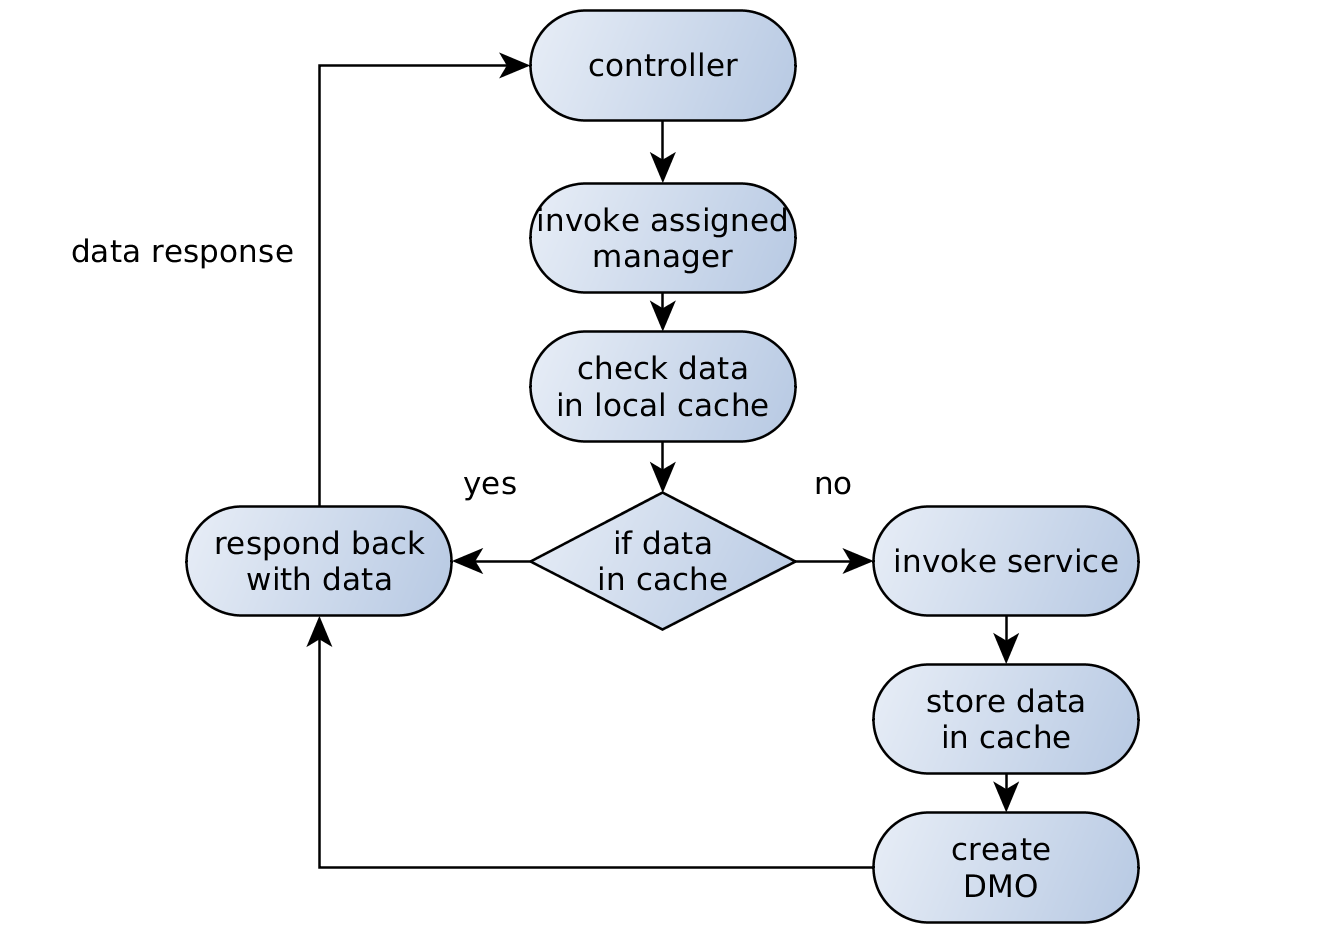
\includegraphics[width=\textwidth]{images/via_manager_1.png}
    \caption{Manager workflow}
    \label{fig:via_manager}
\end{figure}

\begin{figure}[h]
    \centering
	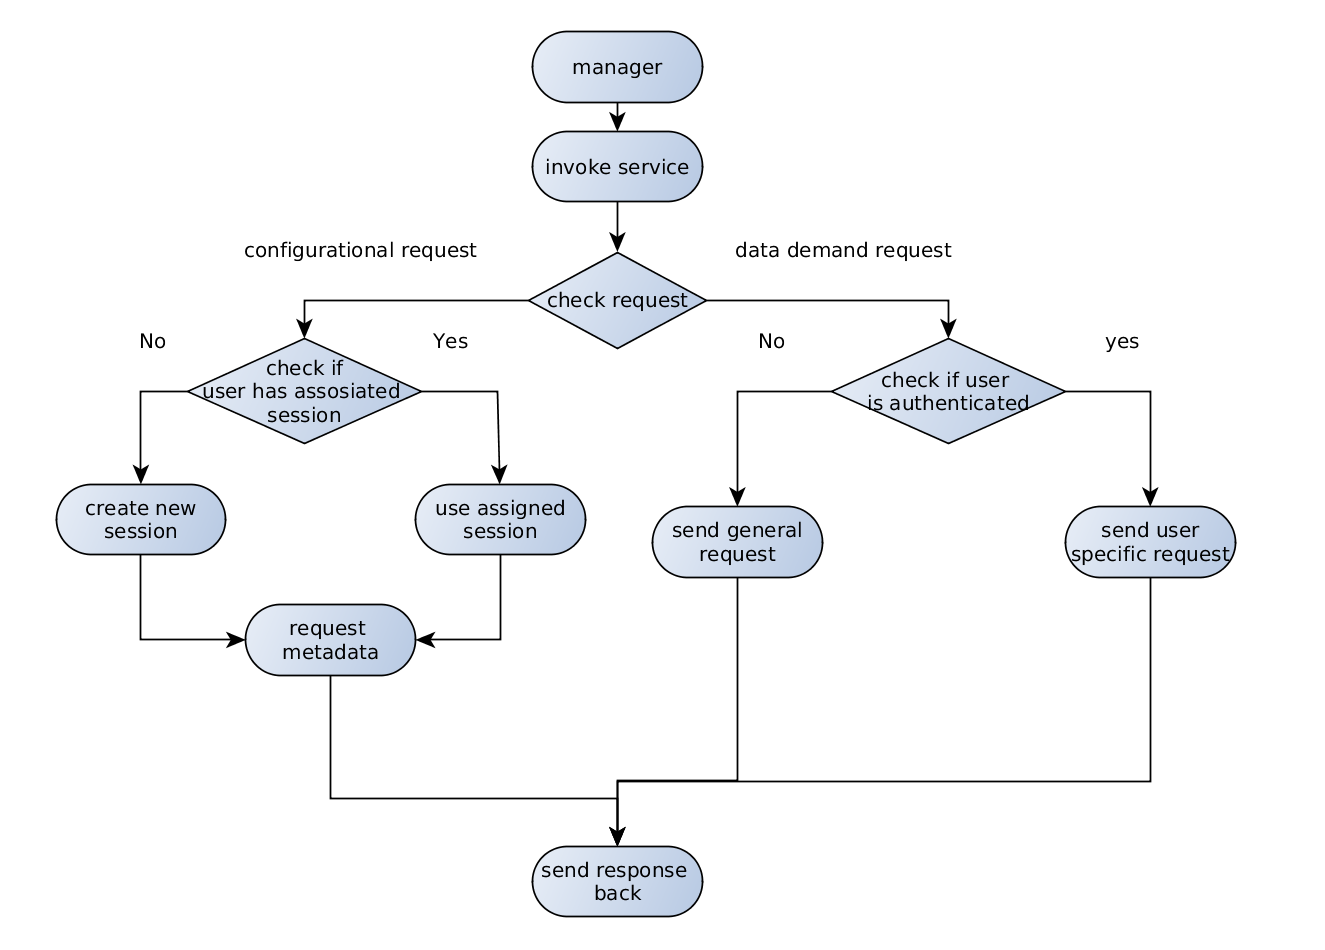
\includegraphics[width=\textwidth]{images/via_service_1.png}
    \caption{Service workflow}
    \label{fig:via_manager}
\end{figure}


\begin{figure}[h]
\begin{center}

	\resizebox{1.0\textwidth}{0.7\textwidth} {

	\begin{sequencediagram}
	\newthread[white]{cl}{Client}
	\newinst[1.7]{cntr}{Controller}
	\newinst[1.3]{mgr}{Manager}
	\newinst[1.3]{lc}{Local Cahce}
	\newinst[1.3]{serv}{Service}
	\newinst[1.3]{es}{External server}

	\begin{call}{cl}{Configuration request}{cntr}{Response}

		\begin{call}{cntr}{Invoke configuation manager}{mgr}{Response Data}
			\begin{call}{mgr}{Check Session key}{lc}{Cache Response}\end{call}
			\begin{sdblock}{alt}{if session key not in cache}
				\begin{call}{mgr}{Get session key using UUID}{serv}{Session key}
					\begin{call}{serv}{Session key request}{es}{Server response}
					\end{call}
				\end{call}
			\end{sdblock}
			\begin{call}{mgr}{Call data service}{serv}{JSON Data}
				\begin{call}{serv}{Call REST API}{es}{JSON data}
				\end{call}
			\end{call}
			\begin{call}{mgr}{Cache response}{lc}{}
			\end{call}
			\begin{call}{mgr}{Make DMO}{mgr}{DMO}\end{call}
		\end{call}

	\end{call}

	\end{sequencediagram}
	}

\end{center}
\caption{Sequence Diagram of Middleware server request process}
\label{fig:arch_uml}
\end{figure}

\begin{figure}[h]
\begin{center}

	\begin{tikzpicture}[
	  font=\sffamily,
	  every matrix/.style={ampersand replacement=\&,column sep=1cm,row sep=2cm},
	  client/.style={draw,thick,ellipse,fill=yellow!20,inner sep=.3cm},
	  middleware/.style={draw,very thick,shape=rectangle,inner sep=.3cm},
	  source/.style={draw,thick,rounded corners,fill=yellow!20,inner sep=.3cm},
	  sink/.style={source,fill=green!20},
	  every node/.style={align=center}]

	  \tikzstyle{state} = [draw, very thick, fill=white, rectangle, minimum height=3em, minimum width=7em, node distance=8em, font={\sffamily\bfseries}]
	  \tikzstyle{stateEdgePortion} = [black,thick];
	  \tikzstyle{stateEdge} = [stateEdgePortion,->];
	  \tikzstyle{edgeLabel} = [pos=0.5, text centered, font={\sffamily\small}];


	  % Position the nodes using a matrix layout
	  \matrix{
	    \& \node[client] (client) {Clients}; \& \\

	    \& \node[middleware] (middleware) {Middleware}; \& \\

	    \node[sink] (mtserver) {Metadata Server};
	      \& \& \node[sink] (ovp) {OVP}; \\
	  };

	  \draw ($(client.south) + (-.5em,0)$) 
	      edge[stateEdge] node[edgeLabel,xshift=-1em, yshift=-1em]{\emph{Request}} 
	      ($(middleware.north) + (-.5em,0)$);
	  \draw ($(middleware.north) + (.5em,0)$) 
	      edge[stateEdge] node[edgeLabel,xshift=4em]{\emph{Data}} 
	      ($(client.south) + (.5em,0)$);


	  \draw ($(middleware.west) + (0,.5em)$) 
	      edge[stateEdge] node[edgeLabel,xshift=-4em, yshift=-1em]{\emph{Request}} 
	      ($(mtserver.north) + (-.5em,0)$);
	  \draw ($(mtserver.north) + (.5em,0)$) 
	      edge[stateEdge] node[edgeLabel,xshift=2em]{\emph{Session ID}} 
	      ($(middleware.west) + (0,-.5em)$);


	  \draw ($(middleware.east) + (0,.5em)$) 
	      edge[stateEdge] node[edgeLabel,xshift=-2em, yshift=-1em]{\emph{Request}} 
	      ($(ovp.north) + (.5em,0)$);
	  \draw ($(ovp.north) + (-.5em,0)$) 
	      edge[stateEdge] node[edgeLabel,xshift=2em]{\emph{Data Resp}} 
	      ($(middleware.east) + (0,-.5em)$);


	\end{tikzpicture}

\end{center}
\caption{Architecture overview}
\label{fig:arch_overview}
\end{figure}


\begin{figure}[h]
\begin{center}

	\resizebox{1.0\textwidth}{0.8\textwidth} {

	\begin{sequencediagram}
	\newthread[white]{cl}{Client}
	\newinst[1.7]{mw}{Middleware}
	\newinst{lc}{Local Cache}
	\newinst[1.9]{ms}{Metadata Server}
	\newinst[1.3]{cs}{Content Server}

	\begin{call}{cl}{First request}{mw}{Response}

		\begin{call}{mw}{Create new session}{ms}{Session ID}
		\end{call}

		\begin{call}{mw}{Cache Session}{lc}{}
		\end{call}

		\begin{call}{mw}{Get content locator}{ms}{URL}
		\end{call}

		\begin{call}{mw}{Cache Locator}{lc}{}
		\end{call}

	\end{call}

	\begin{call}{cl}{GET Request}{mw}{GET Response}
		
		\begin{call}{mw}{Check Local Cache}{lc}{}
		\end{call}

		\begin{sdblock}{alt}{if data in cache}
			\begin{call}{mw}{Send response to Client}{cl}{}
			\end{call}
			\begin{sdblock}{else}{}
				\begin{call}{mw}{Request Content}{cs}{Response}
				\end{call}
				\begin{call}{mw}{Cache content}{lc}{}
				\end{call}
			\end{sdblock}
		\end{sdblock}


	\end{call}

	\end{sequencediagram}
	}

\end{center}
\caption{Sequence Diagram of message exchanging}
\label{fig:arch_uml}
\end{figure}

\newpage
